\subsection{Narzędzia wspierające}

\subsubsection{Git i GitHub}
\begin{wrapfigure}{r}{0.22\textwidth}
  \begin{center}
    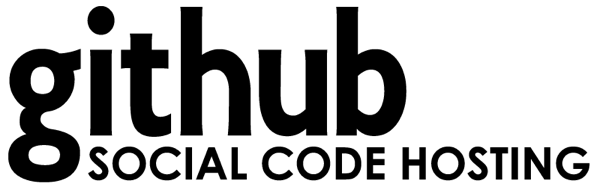
\includegraphics[width=0.2\textwidth]{github}
    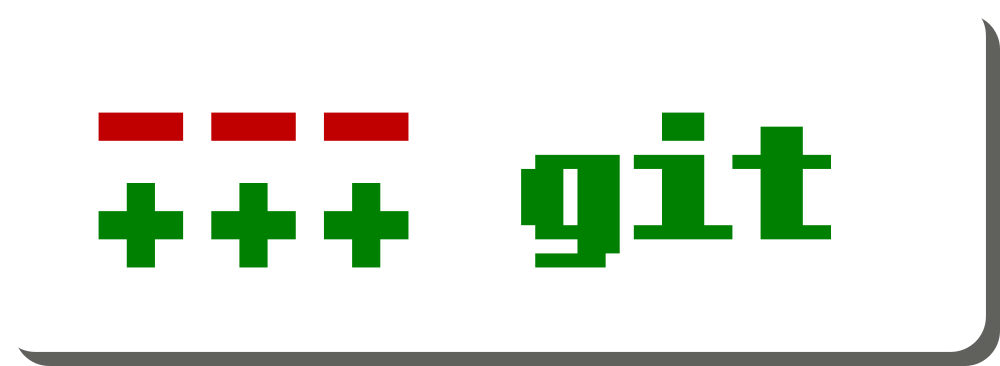
\includegraphics[width=0.2\textwidth]{git}
  \end{center}
\end{wrapfigure}
\textbf{Git} to otwarty rozproszony system kontroli wersji.
Pozwala na łatwe tworzenie i łączenie gałęzi rozwoju projektu, szybkie przemieszczanie się pomiędzy wersjami i sprawdzanie różnic pomiędzy nimi.
\textbf{Git} jest stosowany w takich projektach, jak jądro systemu Linux i umożliwia bardzo wiele (nawet w stosunku do innych nowoczesnych rozproszonych systemów kontroli wersji).
Niestety, powoduje to, że nie jest to system łatwy w nauce.

Zdecydowaliśmy się na system \textbf{Git}, ze względu na doskonały serwis \emph{GitHub}\footnote{\url{http://github.com}}

Serwis \emph{GitHub} posłużył nam nie tylko, jako przestrzeń do współdzielenia kodu.
Serwis ten udostępnia wiele narzędzi, które były bardzo przydatne w czasie prac nad projektem.
Korzystaliśmy z wykresów, które pomagały się zorientować, który członek zespołu co robi.
Inna przydatna opcja, z której korzystaliśmy, aby zapewnić wysoką jakość kodu, to komentowanie kodu napisanego przez innych.
Od kiedy został wprowadzony ulepszony system zadań (\emph{Issues 2.0}), korzystaliśmy z niego w celu przechowywania wymagań i komunikacji z opiekunem projektu.

Ponadto serwis pozwala na automatyczne powiadamianie o nowych zmianach w projekcie na kanale IRC, co było bardzo pomocne~--- motywowało do przeglądania kodu innych i usprawniało integrację.


\subsubsection{Nosetests}
\textbf{Nosetests}, to biblioteka, której używaliśmy do testowania wytwarzanego przez nas oprogramowania.
Biblioteka bazuje na module \texttt{unittest} dostarczanym w standardowej bibliotece języka \textbf{Python}.

Głównym powodem, dla którego zdecydowaliśmy się na korzystanie z tej biblioteki jest jej zdolność do automatycznego dodawania potrzebnych ścieżek.
Ta cecha jest niezbędna do uruchamiania testów bez IDE, a alternatywą jest dopisanie kilku linii, ustawiających ścieżki na prawidłowe w każdym teście.

Ponadto \textbf{Nosetests} udostępnia wiele rozszerzeń, ułatwiających pisanie testów, takich jak generatory testów.
